\newpage
\section{Bestimmung der internen Quanteneffizienz}
\thispagestyle{fancy}
\begin{figure}[h]
    \centering
    \begin{minipage}[t]{0.49\linewidth}
        \centering
        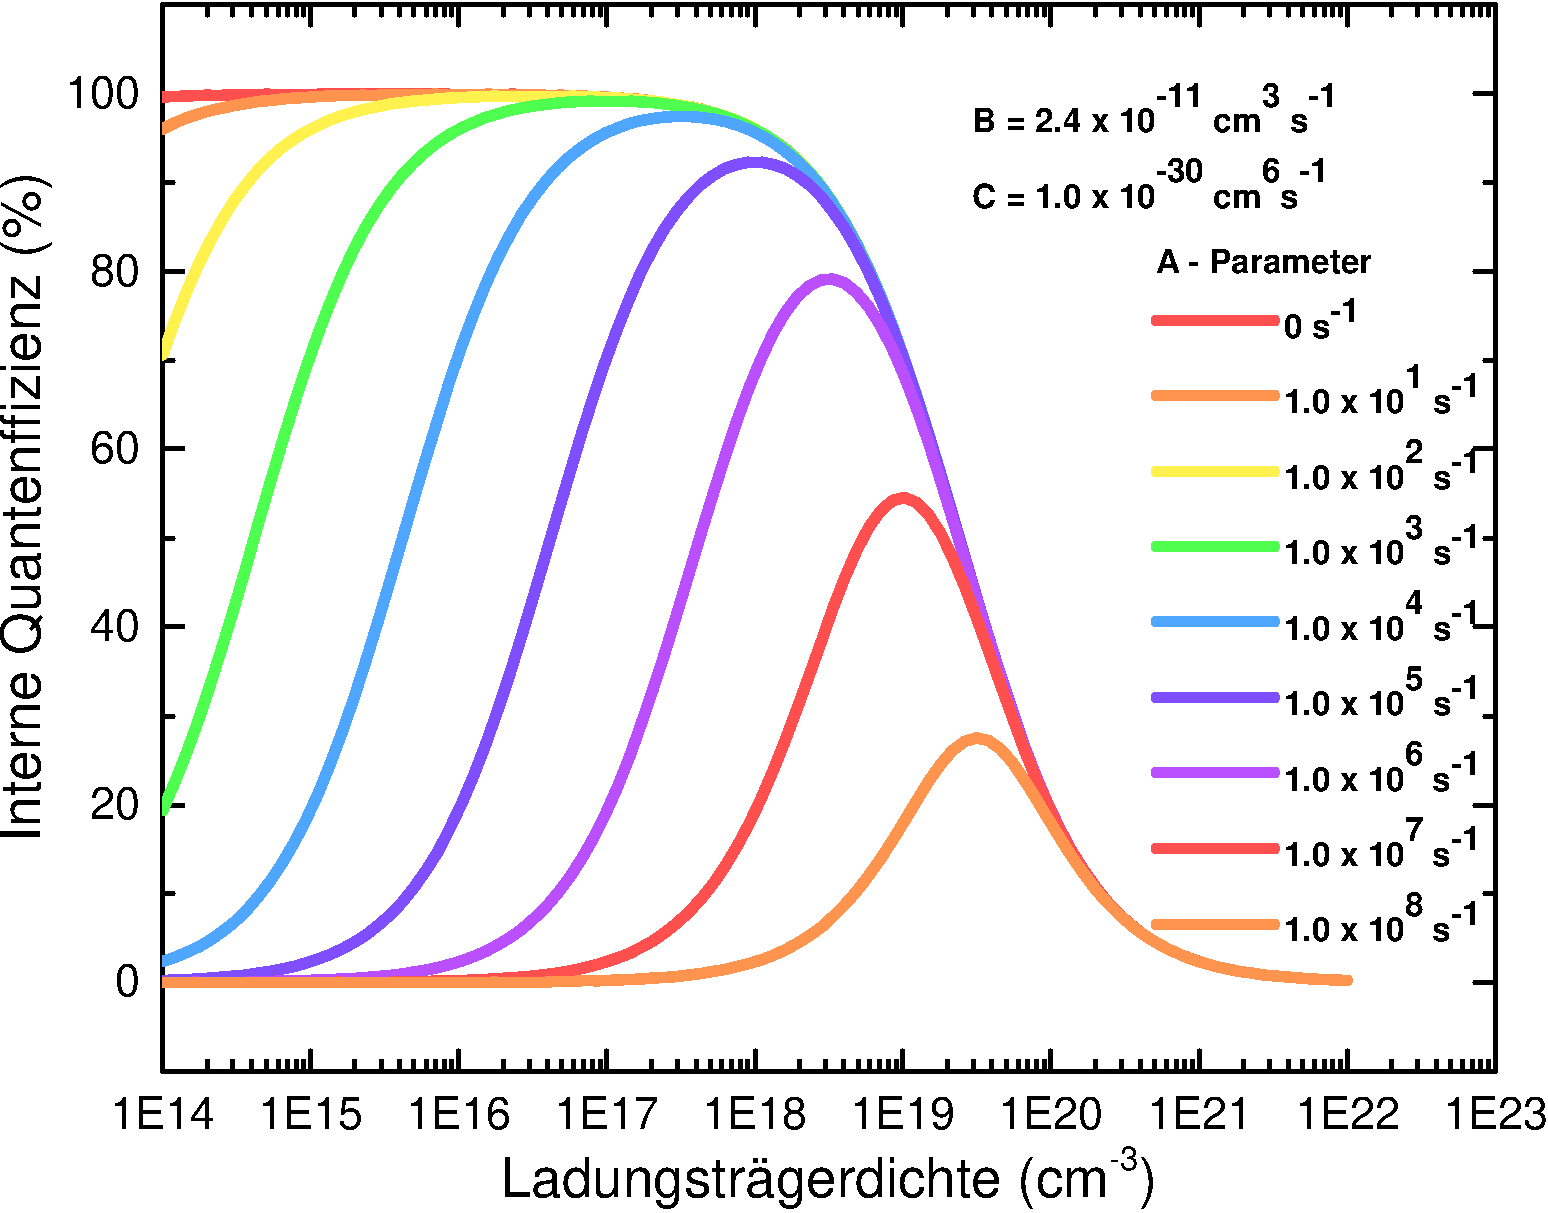
\includegraphics[width=\linewidth]{Bilder/IQEohneDotierungVerschAParams.pdf}
        \caption{Die Grafik zeigt die Abhängigkeit der internen Quanteneffizienz von der Ladungsträgerdichte für feste Paramater B und C. Der Paramater wird A wird variiert mit 9 verschiedenen Werten von $0 s^{-1} $ bis $10^9 s^{-1}$ ~\cite{semreich}.}
        \label{fig:abha}
    \end{minipage}
    \hfill
    \begin{minipage}[t]{0.49\linewidth}
        \centering
        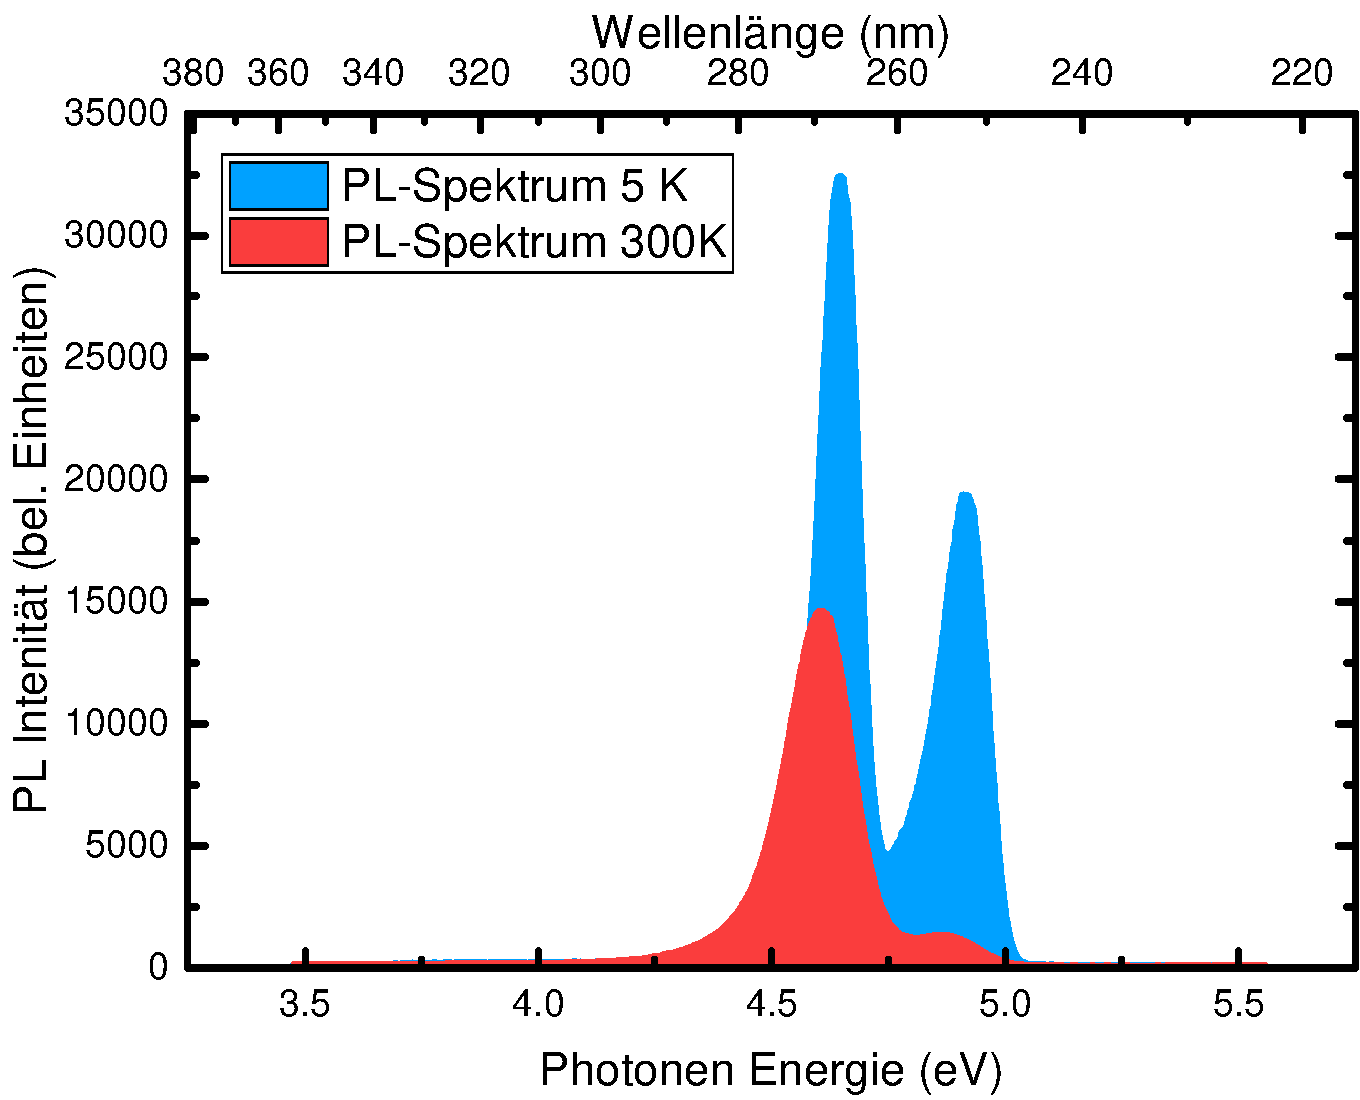
\includegraphics[width=\linewidth]{Bilder/BeispielIQEbestimmen.pdf}
        \caption{Photolumineszenzspektrum bei $5K$ und $300K$. Die integrierte Intensität ist die Fläche des jeweiligen Spektrums.}
        \label{fig:beispielint}
    \end{minipage}% <- sonst wird hier ein Leerzeichen eingefügt
\end{figure}
\raggedright
Die aktive Region einer idealen LED würde für jedes injizierte Elektron jeweils ein Photon aussenden. 
Das bedeutet, die IQE die nach \cite{schub} wie folgt definiert ist
\begin{equation}
    IQE = \frac{ \footnotesize \text{Anzahl der Photonen die von der aktiven Zone emittiert werden pro Sekunde}}{ \footnotesize \text{Anzahl der Elektronen die in die LED injiziert werden pro Sekunde}}
\end{equation}
müsste den Wert $1$ annehmen. Die IQE kann somit analog beschrieben werden als Verhältnis von radiativer Rekombination und der effektiven Rekombination. Beschrieben mit Ratengleichungen und mit \ref{eq:iqe1} ist die IQE in ihrer einfachsten Form somit
\begin{equation}
    IQE = \frac{B \cdot n^2}{A \cdot n + B \cdot n^2 + C \cdot n^3} = \frac{R_{rad}}{R_{eff}}
\end{equation}
Die IQE kann mit Hilfe der Photolumineszenzspektroskopie bestimmt werden, in dem angenommen wird, dass keine thermisch aktivierten Defekte bei Raumtemperatur vorhanden sind
\begin{equation}
    A \propto e^{\frac{-E_{activation}}{kT}}
\end{equation}
Mit dieser und der Annahme das keine Auger Rekombination ($ C \cdot n^3 $) auftritt, ist die IQE bei Tieftemperatur ($ \propto 5K$) gleich 1. Somit kann die IQE beschrieben werden
\begin{equation}
    IQE(T) = \frac{\text{Integrierte PL Intensität (T)}}{ \text{Integrierte PL Intensität } (T \rightarrow 0 K) }
    \label{eq:standardiqe}
\end{equation}
Als Quotient der integrierten PL Intensität bei Temperatur T und integrierter PL Intensität bei Tieftemperatur ($5K$). Die IQE ist folglich abhängig von der Temperatur, da der Paramater A für die SRH-Rekombination temperaturabhängig ist [Abb. \ref{fig:abha}]. 
Um also die IQE bei Raumtemperatur zu bestimmen, wird das Spektrum einer Probe bei 5K und 300K bei ansonsten möglichst gleichen Bedingungen aufgenommen, wie in Abbildung [\ref{fig:beispielint}] exemplarisch dargestellt ist . Die Intensität in Abhängigkeit der Wellenlänge wird interpoliert, dann integriert und dann das Verhältnis berechnet. 
%